\section{2D model}

Two models for a 2-dimensional scheme are proposed. The first considers height and width, while the second considers width and depth. The main difference is that in the first model, the neurotransmitters need to travel a distance before reaching the receptors. While in the second model the neurotransmitters and receptors start side by side.


\subsubsection{Numerical scheme}
We use the finite difference method to discretize the modeling equation (\ref{eq:diffusion}), with boundary conditions (\ref{eq:changeInConcentration}) and (\ref{eq:changeInPR}).
%$$   
\begin{align} \label{equ:2dscheme}
C_{j,k}^{i+1}=&C_{j,k}^{i}+\frac{\Delta t}{2} \Bigg[\kappa \Big(\frac{C_{j+1,k}^{i} -2C_{j,k}^{i} + C_{j-1,k}^{i}}{(\Delta y)^2} +\frac{C_{j,k+1}^{i} -2C_{j,k}^{i} + C_{j,k-1}^{i}}{(\Delta x)^2}\Big)\nonumber\\
&-k_{1}C_{j,k}^i P_{j,k}^i+k_{2}(1-P_{j,k}^i)\Bigg]  \\
P_{j,k}^{i+1}&=P_{j,k}^i + \Delta t \Big[-k_{1}C_{j,k}^iP_{j,k}^i+k_{2}(1-P_{j,k}^i) \Big],
\end{align}  
where $i$ is points in time, and $j$, $k$ are points in space. $ \Delta t $, $ \Delta x $, $ \Delta y $ are step length in time, width and height or depth, respectively.

\subsection{Height and width}
%Here a 2-dimensional model for the neurotransmitters diffusing from the axon terminal to the dendrite spine.

\subsubsection{Domain, initial and boundary values} \label{2DdiffHeightwidth}
We consider the synaptic cleft a square with height $L$ and width $2R$.
We assume initially that the neurotransmitters are uniformly distributed on the axon terminal, at height $y = L$, and the receptors are uniformly distributed on the dendritic spine, $y=0$. We also assume that the surface of the dendritic spine is covered by an extracellular fluid with thickness $\epsilon$ as presented in the 1D case in figure \ref{fig:model_1d}.

Like in the 1D-model, the neurotransmitters in this area can only react with unoccupied receptors. 

\subsubsection{Results}
Using the 5-point-formula in equation (\ref{equ:2dscheme}), what was proposed in \ref{2DdiffHeightwidth} was attempted, but the system was numerically unstable. Therefore, it will not be included in this report. 


\subsection{Width and depth}

\subsubsection{Domain, initial and boundary values}

Initially we chose a random point where we released all the neurotransmitters. The initial function for the concentration of neurotransmitters is zero everywhere except from that point. On the boundary we assumed that the particles could freely diffuse outside of the domain.

To simplify the diffusion equation we neglect the height of the synaptic cleft. Furthermore, we chose to view the resulting disc as a square with size $4R^2$, due to the difficult nature of the Laplacian in cylindrical coordinates. We assume that the receptors are equally distributed over the square.

If the number of bounded receptors doesn't change over a time interval $\Delta t$, we assume equilibrium and that a signal is being transmitted. 



\subsubsection{Results}
The program \textit{dim2.m} was used with values given in \cite{task}, with $k_1=10^4$, $k_2=10$, and 
\begin{itemize}
\item number of steps in $x$- and $y$-direction, $n_x=n_y=10$
\item number of time steps $n_t=4\cdot 10^5$, simulated over 1 second
\end{itemize}
This results in a signaling time of $t_s=33.8$ms. The following figures show the distribution of neurotransmitters and free receptors at the signaling time. 

\begin{figure}[ht]
    \centering
    \begin{subfigure}[b]{0.45\textwidth}
        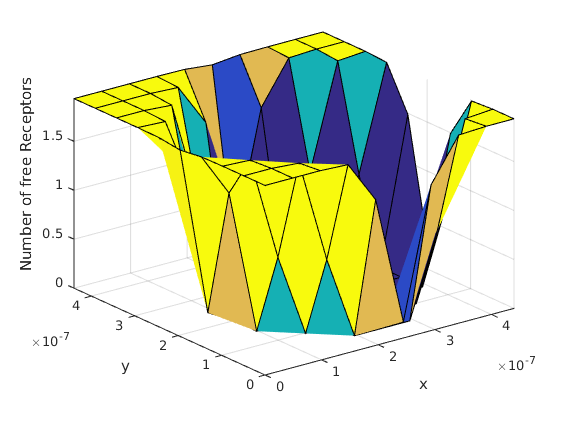
\includegraphics[width=\textwidth]{receptordensity5ms}
        \caption{Distribution of free receptors at 5 ms.}
    \end{subfigure}
    ~ 
    \begin{subfigure}[b]{0.45\textwidth}
        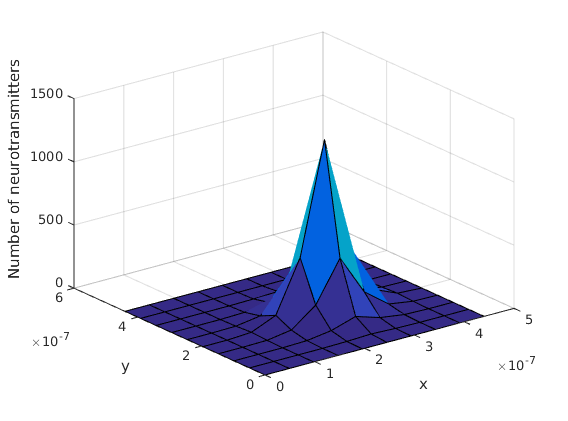
\includegraphics[width=\textwidth]{distneurottansmitters5ms}
        \caption{Distribution of neurotransmitters at 5 ms.}
    \end{subfigure}

    \begin{subfigure}[b]{0.45\textwidth}
        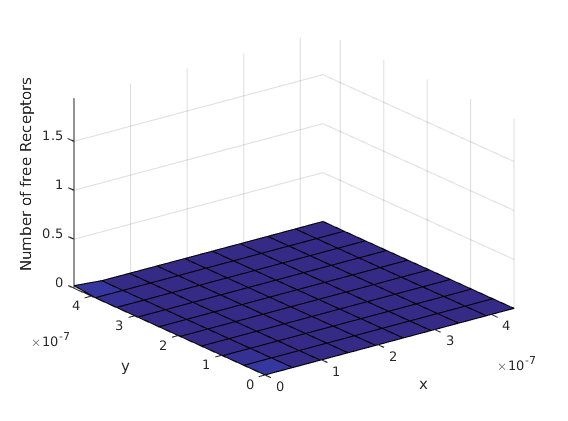
\includegraphics[width=\textwidth]{receptordensity}
        \caption{Distribution of free receptors at signal time.}
        \label{fig:receptordensitysignaltime}
    \end{subfigure}
    ~
    \begin{subfigure}[b]{0.45\textwidth}
        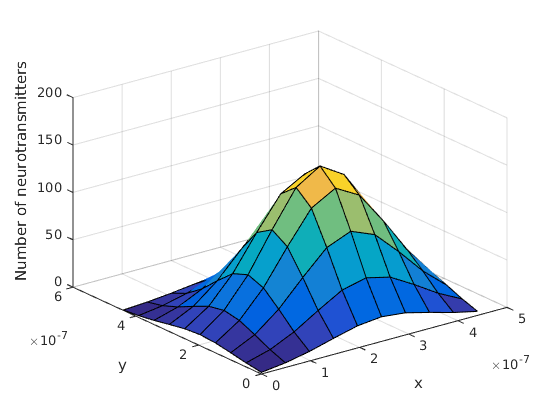
\includegraphics[width=\textwidth]{distneurottansmitters}
        \caption{Distribution of neurotransmitters at signal time.}
        \label{fig:concentrationOfReceptors2d}
    \end{subfigure}    
    
    \caption{Simulation of the synaptic cleft at different times. This model is in 2 dimensions, ignoring height. In (a) and (c) the $z$-axis represents the number of free receptors. In (b) and (d) it represents the number of neurotransmitters.  Signaling time is 33.8 ms.}
\end{figure}

\subsubsection{Discussion}
As we can see from figure \ref{fig:receptordensitysignaltime}, practically all receptors are bounded at this time, so this may be considered an upper bound for the signaling time. This is a two dimensional model, and thus lacks a certain accuracy. %Given more time the model could have been extended to three dimensions, but as a simple representation of what happens during neurotransmission in the synaptic cleft, we consider this model is applicable.\\ Given more time, this model could also have been used to model the clearance time.